\section{Proposed Solution}
\subsection{Core Technologies}
It is proposed that the web platform will be built with React/NextJS, and Material UI/Material Kit. These technologies and libraries are an abstraction of the basic web technology: HTML, CSS, and JS. that allows reduction of development time and costs in creating websites that are responsive, engaging, and informative. The design configuration will come from Material UI/Material Kit with content structure and rendering to be done with React/NextJS. The web platform built by these technologies be deployed in a docker container in the SHL Arya VPS Server.The technologies React/NextJS, and Material UI/Material Kit is open-source and MIT license - allows the use of software for any purpose which allows these technologies to be used in this context.

\subsubsection{React/NextJS}
React is a popular frontend technology to create website divided into components and utilizes client-side rendering to allow fast loading speed with the trade-off of slower initial load speed (NFR2 - Speed). 

The division of UI into components allows easier re-usability of UI components such as a header and a footer that appears in every page, and allow easy to change for update - "one change, change it all" (NFR4 - Maintenance and Extensibility).

The main power of React is the ecosystem and libraries that are available on top of it such as NextJS and Material UI which can ultimately cut the development speed, and allows easier upgrade than other technologies (NFR5 - Maintenance and Extensibility). Two of the common technology used with React is Babel Transpiler for cross-compatibility (NFR1 - Responsive and Compatible) and webpack bundler/minifier for lower bundle or required downloads size (NFR2 - Speed).

NextJS is a library for React that allow server-side static web generation, handling web routes, and code splitting. Server-side static web generation allows the processing of HTML, CSS and JS in the server for the initial serving of web content, and allows web crawlers to read content. Furthermore, NextJS handles web routing with hot reloading - loading only components that has not been downloaded by the browser to allow fast navigation (NFR2 - Speed). Code Splitting is used by NextJS to allows faster initial load speed by only loading code that will be used for the initial session (NFR2 - Speed). 

\subsubsection{Material UI/Material Kit}
NFR4 - User Engagement and Experience is one of the most important requirement of a website, but may take a lot of time to develop. CSS libraries allows cutting the development time for design such as Material UI that contains ready-to-use UI components that are responsive (NFR1 - Responsive and Compatible),  excellent in design (NFR4 - User Engagement and Experience), easy to use, and extensible (NFR5 - Maintenance and Extensibility).

Material Kit is an extension of Material UI that provides a base template for few pages, and a package of configuration for the most common UI component (NFR4 - User Engagement and Experience).

\subsubsection{Docker}
Docker is a deployment technology that allows virtualization in a server to allow the packaging of software into containers for deployment. To satisfy NFR6 - Deployability, the web platform will use docker to allow the deployment through the SHL Arya VPS Server.

\subsubsection{Code Style and Quality}
Written code, especially JS, will conform to the applicable Google Style Guide, as found on \url{https://google.github.io/styleguide/} (NRR5 - Maintenance and Extensibility).

Written code will be reviewed in accordance to the System Health Lab code-review procedures after the deployment of the web platform.

\subsubsection{Code Storage and Development Control}
Git source control will be used, using the remote UWA System Health Lab organisational GitHub (NFR5 - Maintenace and Extensibility).

\subsection{Screenshots} \label{subsec:UISection}
These screenshots represent one possible appearance of the system after the completion of the web platform. However these designs will continually be improved and tweaked during the development process, and primarily serves to illustrate the overall feel of the web platform alongside prototyping page flow.

\sloppy The UI design can be found here: \\ \url{https://www.figma.com/proto/QkvtbwtsiHFUMkQSp8uBQO/Living-Lab-Wireframe?node-id=76%3A1362&viewport=857%2C663%2C0.05884827673435211&scaling=min-zoom}

Select screenshots can be found in Appendix \ref{appendixa}

\subsection{Execution Team}
The development of the web platform will be performed by \textbf{Frinze Erin Lapuz}. \textbf{Caitlin Woods} will provide advice on the development and will run code reviews. \textbf{Eddie Atkinson} will handle the deployment stage after development. \textbf{Professor Melinda Hodkiewicz}, \textbf{Craig Hook}, \textbf{Tamryn Barker}, \textbf{Drew Georgiades} and the rest of the \textbf{Living Lab Team} will provide content for the web platform.

\pagebreak

\appendix
\section {Screenshot} \label{appendixa}

% Page 1-4
\begin{figure}[H]
    \centering
    \begin{minipage}{0.45\textwidth}
        \centering
        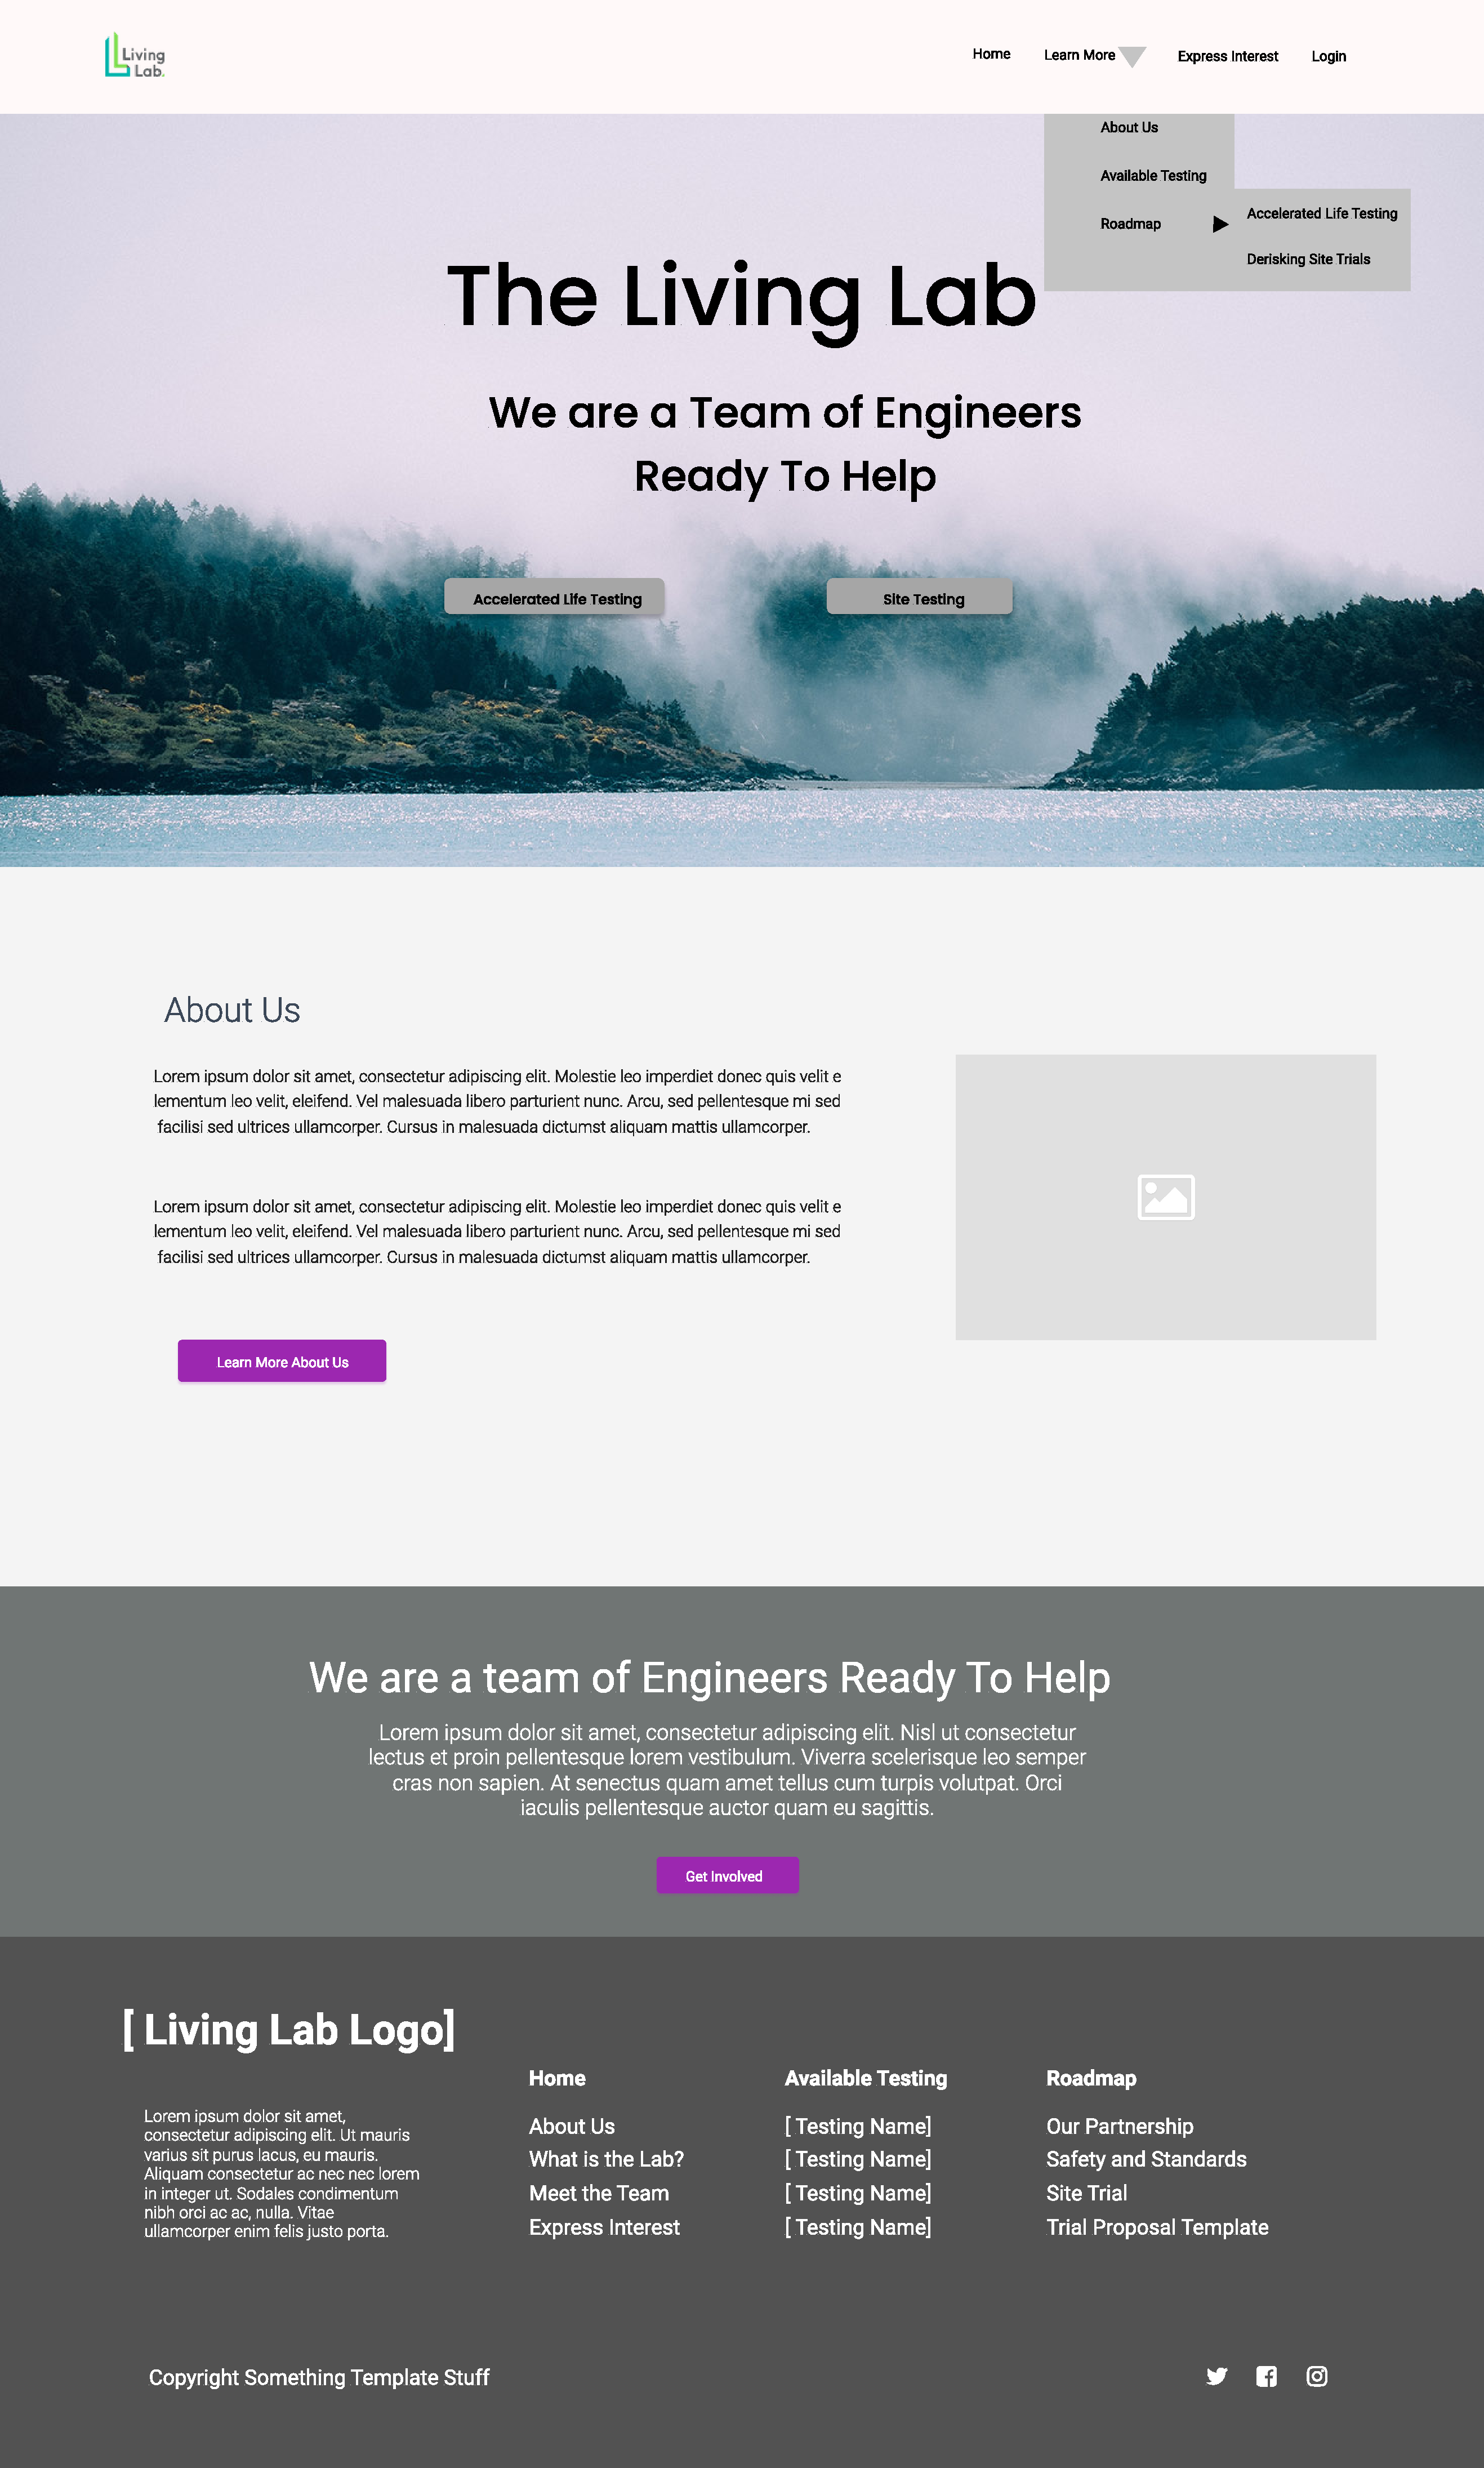
\includegraphics[height=0.4\textheight,page=1]{ProposedSolution/Screenshots.pdf} 
        \caption{Home/Main Page}
    \end{minipage}\hfill
    \begin{minipage}{0.45\textwidth}
        \centering
        \includegraphics[height=0.4\textheight,page=2]{ProposedSolution/Screenshots.pdf} 
        \caption{About Us/Learn More Page}
    \end{minipage}
    \centering
    \begin{minipage}{0.45\textwidth}
        \centering
        \includegraphics[height=0.4\textheight,page=3]{ProposedSolution/Screenshots.pdf} 
        \caption{Contact Page}
    \end{minipage}\hfill
    \begin{minipage}{0.45\textwidth}
        \centering
        \includegraphics[height=0.4\textheight,page=4]{ProposedSolution/Screenshots.pdf} 
        \caption{Contact Modal/Popup (Alternative)}
    \end{minipage}
\end{figure}

% Page 5-8
\begin{figure}[H]
    \centering
    \begin{minipage}{0.45\textwidth}
        \centering
        \includegraphics[height=0.4\textheight,page=7]{ProposedSolution/Screenshots.pdf} 
        \caption{Roadmap Showcase Page}
    \end{minipage}\hfill
    \begin{minipage}{0.45\textwidth}
        \centering
        \includegraphics[height=0.4\textheight,page=8]{ProposedSolution/Screenshots.pdf} 
        \caption{An Example of A Roadmap (Plain Listing Method)}
    \end{minipage}
    \centering
    \begin{minipage}{0.45\textwidth}
        \centering
        \includegraphics[height=0.4\textheight,page=9]{ProposedSolution/Screenshots.pdf} 
        \caption{An Example of A Roadmap (Listing Accordion Method)}
    \end{minipage}\hfill
    \begin{minipage}{0.45\textwidth}
        \centering
        \includegraphics[height=0.4\textheight,page=10]{ProposedSolution/Screenshots.pdf} 
        \caption{An Example of A Roadmap (Card Design)}
    \end{minipage}
\end{figure}

\begin{figure}[H]
    \centering
    \begin{minipage}{0.45\textwidth}
        \centering
        \includegraphics[height=0.4\textheight,page=14]{ProposedSolution/Screenshots.pdf} 
        \caption{Accelerated Life Testing Overview - Vertical Roadmap}
    \end{minipage}
    \centering
    \begin{minipage}{0.45\textwidth}
        \centering
        \includegraphics[height=0.4\textheight,page=15]{ProposedSolution/Screenshots.pdf} 
        \caption{Derisking Site Trials Overview - Vertical Roadmap}
    \end{minipage}\hfill
    \begin{minipage}{0.45\textwidth}
        \centering
        \includegraphics[height=0.4\textheight,page=16]{ProposedSolution/Screenshots.pdf} 
        \caption{Testing Equipment Listing - Picture Card Listing}
    \end{minipage}
    \centering
    \begin{minipage}{0.45\textwidth}
        \centering
        \includegraphics[height=0.4\textheight,page=17]{ProposedSolution/Screenshots.pdf} 
        \caption{Testing Equipment Listing - Picture Card Overlay Listing}
    \end{minipage}\hfill
\end{figure}
\begin{figure}[H]
    \begin{minipage}{0.45\textwidth}
        \centering
        \includegraphics[height=0.4\textheight,page=18]{ProposedSolution/Screenshots.pdf} 
        \caption{Testing Equipment Modal View}
    \end{minipage}
    \centering
    \begin{minipage}{0.45\textwidth}
        \centering
        \includegraphics[height=0.4\textheight,page=19]{ProposedSolution/Screenshots.pdf} 
        \caption{Testing Equipment Page View}
    \end{minipage}\hfill
\end{figure}